% Cartas y Atlas - Parametrización local de variedades
% Compilar con: pdflatex charts_atlas.tex
\documentclass[tikz,border=10pt]{standalone}
\usepackage{tikz}
\usepackage{amsmath,amssymb}
\usetikzlibrary{arrows.meta, positioning, decorations.pathmorphing, calc, patterns}

\definecolor{gdlblue}{RGB}{41, 98, 168}
\definecolor{gdlred}{RGB}{191, 49, 49}
\definecolor{gdlgreen}{RGB}{30, 130, 76}
\definecolor{gdlorange}{RGB}{217, 130, 30}
\definecolor{gdlpurple}{RGB}{118, 56, 138}
\definecolor{gdlgray}{RGB}{140, 140, 140}
\definecolor{gdlyellow}{RGB}{190, 140, 10}

\begin{document}
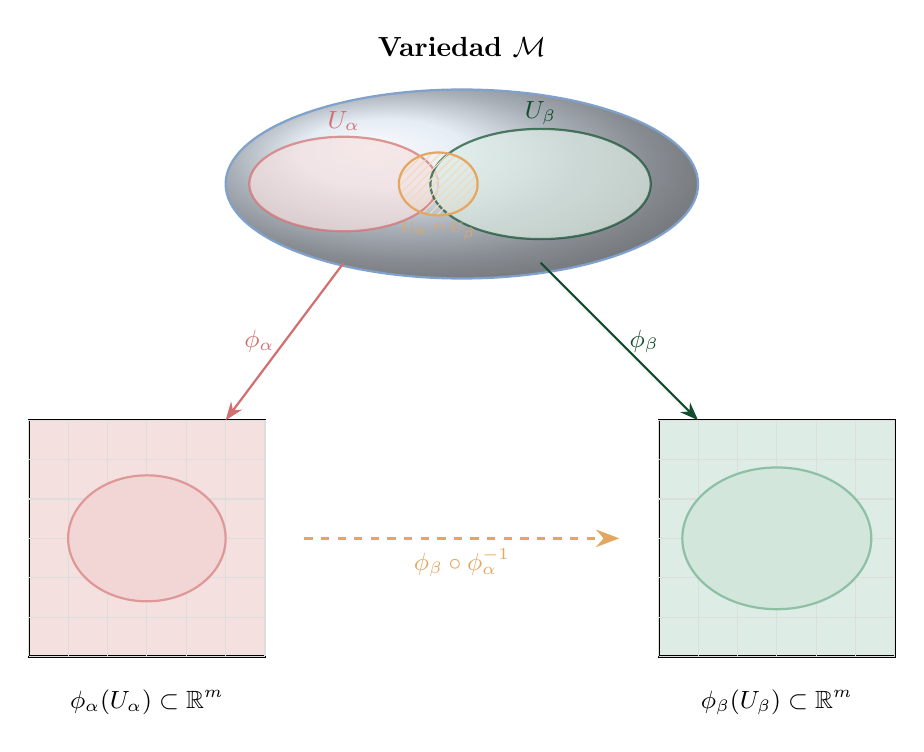
\begin{tikzpicture}[>=Stealth]

% === Variedad M (esfera aplanada) ===
\begin{scope}[shift={(0,3)}]
    \shade[ball color=gdlblue!20, opacity=0.8] (0,0) ellipse (3cm and 1.2cm);
    \draw[thick, gdlblue!60] (0,0) ellipse (3cm and 1.2cm);
    \node[above] at (0, 1.5) {\textbf{Variedad $\mathcal{M}$}};

    % Regiones U_α y U_β
    \draw[thick, gdlred!70, fill=gdlred!15, opacity=0.7] (-1.5,0) ellipse (1.2cm and 0.6cm);
    \node[gdlred!70, font=\small] at (-1.5, 0.8) {$U_\alpha$};

    \draw[thick, gdlgreen!60!black, fill=gdlgreen!15, opacity=0.7] (1,0) ellipse (1.4cm and 0.7cm);
    \node[gdlgreen!60!black, font=\small] at (1, 0.9) {$U_\beta$};

    % Intersección
    \draw[thick, gdlorange!70, pattern=north east lines, pattern color=gdlorange!30]
        (-0.3,0) ellipse (0.5cm and 0.4cm);
    \node[gdlorange!70, font=\tiny] at (-0.3, -0.6) {$U_\alpha \cap U_\beta$};
\end{scope}

% === Cartas (planos euclidianos) ===
% Carta φ_α
\begin{scope}[shift={(-4,-1.5)}]
    \draw[thick, fill=gdlred!15] (-1.5,-1.5) rectangle (1.5,1.5);
    \draw[gdlgray!30, step=0.5] (-1.5,-1.5) grid (1.5,1.5);
    \node[below, font=\small] at (0, -1.8) {$\phi_\alpha(U_\alpha) \subset \mathbb{R}^m$};

    % Región mapeada
    \draw[thick, gdlred!50, fill=gdlred!20] (0,0) ellipse (1cm and 0.8cm);
\end{scope}

% Carta φ_β
\begin{scope}[shift={(4,-1.5)}]
    \draw[thick, fill=gdlgreen!15] (-1.5,-1.5) rectangle (1.5,1.5);
    \draw[gdlgray!30, step=0.5] (-1.5,-1.5) grid (1.5,1.5);
    \node[below, font=\small] at (0, -1.8) {$\phi_\beta(U_\beta) \subset \mathbb{R}^m$};

    % Región mapeada
    \draw[thick, gdlgreen!50, fill=gdlgreen!20] (0,0) ellipse (1.2cm and 0.9cm);
\end{scope}

% === Flechas ===
% φ_α
\draw[->, thick, gdlred!70] (-1.5, 2) -- node[left, font=\small] {$\phi_\alpha$} (-3, 0);

% φ_β
\draw[->, thick, gdlgreen!60!black] (1, 2) -- node[right, font=\small] {$\phi_\beta$} (3, 0);

% Función de transición
\draw[->, very thick, gdlorange!70, dashed] (-2, -1.5) -- node[below, font=\small] {$\phi_\beta \circ \phi_\alpha^{-1}$} (2, -1.5);

\end{tikzpicture}
\end{document}
